%\FloatBarrier
\section{Milestone II}\label{sec:milestone_2}
With fundamental cosmology established in sec. \ref{sec:milestone_1}, we can now describe the baseline or so-called "background" behaviour of our universe, with a relatively simple evolution of cosmological parameters as the universe expands (refer fig. \ref{fig:milestone_1_Omega_i_of_x}). Now we wish to look backwards from our current time, and compute the path of photons travelling towards a current-day observer from the early universe.

In order to study the behaviour of photons and thermal evolution of the early universe, we consider it to be a large continuous fluid, specifically a hot plasma. The thermodynamics and statistical mechanics for this are described in \citet[chap.~3]{baumannLectureNotesCosmology2017} and \citet[chap.~3, 4]{dodelsonModernCosmology2003}, while the specific Boltzmann formalism utilized is that of \citet{wintherCosmologyIILecture2024}, \href{https://cmb.wintherscoming.no/theory_thermodynamics.php#thermo}{available here}.

\subsection{Theory}
Considering the early universe, there are three main interactions between particle species of interest, Couloumb scattering (\ref{eq:couloumb_scattering}), Thomson scattering (\ref{eq:thomson_scattering}), and the formation/ionization of Hydrogen (\ref{eq:hydrogen_capture}).

\begin{align}
e^- + p^+ &\rightleftharpoons e^- + p^+ \label{eq:couloumb_scattering} \\
e^- + \gamma &\rightleftharpoons e^- + \gamma \label{eq:thomson_scattering} \\
e^- + p^+ &\rightleftharpoons H + \gamma \label{eq:hydrogen_capture}
\end{align}

Start with eqs. \ref{eq:tau_integral} \citep[sec.~4.4]{dodelsonModernCosmology2003} and \ref{eq:tau_ODE}.

\begin{equation}\label{eq:tau_integral}
\tau(\eta) = \int_{\eta}^{\eta_0} n_e \sigma_T a d\eta' \quad \text{[dimensionless]}
\end{equation}

\begin{equation}\label{eq:tau_ODE}
\boxed{\tau' = \frac{d\tau}{dx} = -\frac{c n_e \sigma_T }{H}} \quad \text{[dimensionless]}
\end{equation}

Also the visibility function \ref{eq:visibility_function}.

\begin{equation}\label{eq:visibility_function}
\tilde{g}(x) = \frac{d}{dx}e^{-\tau} = -\tau' e^{-\tau}, \quad \text{by def.} \int_{-\infty}^{0} \tilde{g}(x)dx = 1
\end{equation}

We wish to compute the fractional electron density given by \ref{eq:fractional_electron_density}, where we assume all baryons are protons and there are no heavier elements. This approximation is acceptable for getting a simple reionization with clear falloff of electrons as they get absorbed into hydrogen atoms. By including ionization into Helium, our resulting ionization plot would have multiple bumps for ionization into different states of Hydrogen+Helium.


\begin{equation}\label{eq:fractional_electron_density}
\boxed{X_e \equiv n_e / n_H}\,, \text{ with } \,\, n_H = n_b \approx \frac{\rho_b}{m_H} = \frac{\Omega_{b0} \rho_{c0}}{m_H a^3}
\end{equation}


In order to calculate the electron density, we can use the Saha approximation given in eq. \ref{eq:saha_approx}. This is valid for large temperatures $T$, early in the universe. However, as the temperature falls the Saha approximation continues to predict a simple exponential decay of free electrons as they all become bound to hydrogen (and heavier elements), but this assumes the interaction \ref{eq:hydrogen_capture} continues to be perfectly efficient, which is not the case in practice. See fig. 3.8 in \citet[sec. 3.3.3]{baumannLectureNotesCosmology2017}. We seek to recreate this figure with a numerical simulation.

\begin{equation}\label{eq:saha_approx}
\begin{aligned}
\Aboxed{\frac{X_e^2}{1-X_e} = \frac{1}{n_b} \left(\frac{m_e T_b}{2\pi}\right)^{3/2} e^{-\frac{\epsilon_0}{k_b T_b}}} \quad [X_e \; \rm dimensionless]
\end{aligned}
\end{equation}

In order to properly simulate the change in electron density, we can switch to the more accurate Peebles equation given as eq. \ref{eq:peebles_equation} \citep{peeblesRecombinationPrimevalPlasma1968,zeldovichRecombinationHydrogenHot1969}, with supporting definitions in eq. \ref{eq:peebles_quantities_definition}. This equation is numerically unstable when solved for very large $T$ (early on), but is perfectly appropriate around when the Saha approximation stops being accurate.

\begin{equation}\label{eq:peebles_equation}
\begin{aligned}
\boxed{\frac{dX_e}{dx} = \frac{C_r(T_b)}{H} \left[\beta(T_b)(1-X_e) - n_H \alpha^{(2)}(T_b)X_e^2\right]} \\
{[X_e \; \rm dimensionless]}
\end{aligned}
\end{equation}

We will also calculate the so-called "sound horizon at decoupling", the total distance a sound-wave in the primordial photon-baryon plasma can propagate from the Big Bang until photons decouple. Pure photons have a sound speed $c/\sqrt{3}$, while sound-waves in the primordial plasma follow the slightly lower $c_s = c \sqrt{\frac{R}{3(1+R)}}$, with $R = \frac{4\Omega_{\gamma 0}}{3\Omega_{b 0} a}$. Thus we end up with the sound-horizon given in eq. \ref{eq:sound_horizon}.

\begin{equation}\label{eq:sound_horizon}
\begin{aligned}
\Aboxed{s(x) &= \int_0^{a} \frac{c_s dt}{a} = \int_{-\infty}^{x} \frac{c_s dx}{\mathcal{H}} \to \frac{ds(x)}{dx} = \frac{c_s}{\mathcal{H}}}\:,\\
\text{with}\,\,\,&s(x_{\rm ini}) = \frac{c_s(x_{\rm ini})}{\mathcal{H}(x_{\rm ini})} \quad {\text{[unit \unit{m}]}}
\end{aligned}
\end{equation}


\subsection{Implementation details}
%Something about the numerical work.

\subsection{Results}
See figs. \ref{fig:milestone_2_Xe}, \ref{fig:milestone_2_tau_and_derivs}, \ref{fig:milestone_2_g_tilde}, \ref{fig:milestone_2_g_tilde_deriv}, \ref{fig:milestone_2_g_tilde_double_deriv}.

Simulated recombination happens at $x = -3.452$, giving a recombination time (cosmic time) of $96\, 273\, 898.543$ years. This corresponds to a redshift $z = 33.908$. However, the actual expected redshift should be $z=1100$, and the age of the universe $378\, 000$ years, so this is extremely late. This is also visible from plots like fig. \ref{fig:milestone_2_Xe}. I have not figured out where the bug is for this one, but it affects all later plots.

\begin{figure}[h!tbp]
\centering
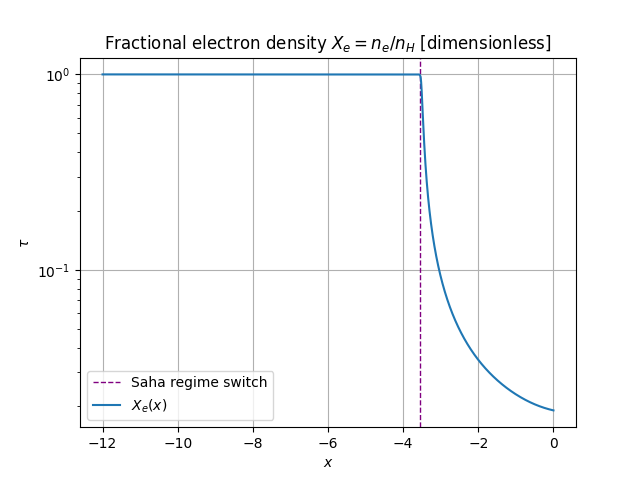
\includegraphics[width=0.4\textwidth]{../Milestone 2/Plots/Xe.png}
\caption{Fractional electron density. Early times with density about 1 correspond to a high-energy universe where any hydrogen that forms instantly gets reionized by random photons. We see the expected exponential drop once the temperature has dropped sufficiently and recombination kicks in, with the dampening provided by Peebles making $X_e$ converge to some non-zero value as the likelihood of proton-electron interactions drop. This would not be modelled by a simple implementation of just the Saha approximation. However, the extremely late recombination is unexpected, so the electron fraction does not seem to have stabilized by the present day which cannot be correct.}
\label{fig:milestone_2_Xe}
\end{figure}

\begin{figure}[h!tbp]
\centering
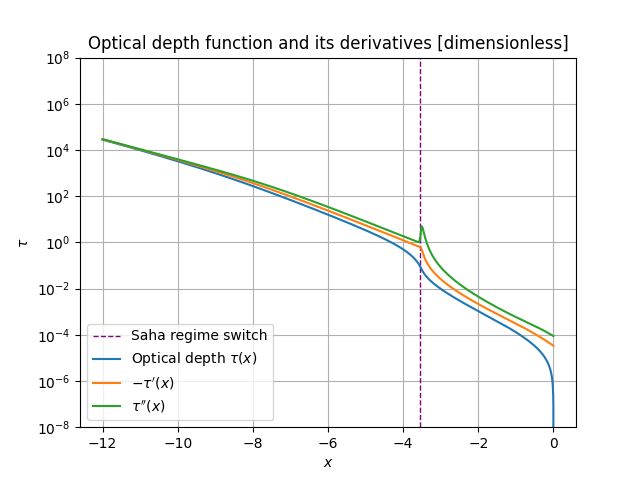
\includegraphics[width=0.4\textwidth]{../Milestone 2/Plots/tau_and_derivs.png}
\caption{The optical depth function and its derivatives, which evolves as expected, falling steadily as the universe expands until recombination, which is adequately represented by the point where we switch from the Saha approximation, noted in the plot. The bump in optical density is provided by all the new hydrogen forming. However, the falloff once the universe becomes transparent is not as sharp as expected, and recombination happens too late anyway.}
\label{fig:milestone_2_tau_and_derivs}
\end{figure}

\begin{figure}[h!tbp]
\centering
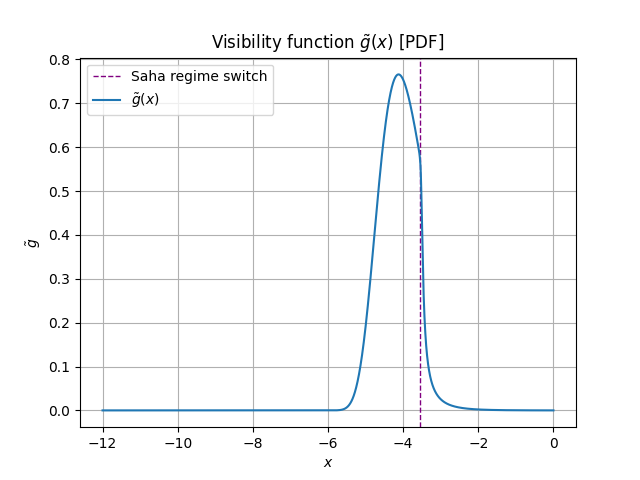
\includegraphics[width=0.4\textwidth]{../Milestone 2/Plots/g_tilde.png}
\caption{The visibility function is a probability density function (and thus the integral sums to 1, which lines up with what we see), and represents the likelihood that a photon was last scattered at time $x$ before free flying to hit a modern-day observer. The clear peak corresponds to recombination, where the universe becomes transparent as free electrons are bound into hydrogen, and represents the surface of last scattering. It is very unlikely that photons before this point flew unimpeded, as they likely scattered off the dense medium before this (see fig. \ref{fig:milestone_2_tau_and_derivs}). However, the peak is not quite as defined as expected.}
\label{fig:milestone_2_g_tilde}
\end{figure}

\begin{figure}[h!tbp]
\centering
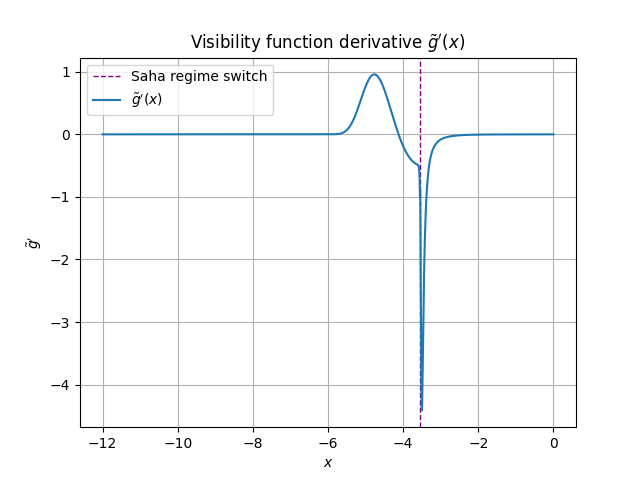
\includegraphics[width=0.4\textwidth]{../Milestone 2/Plots/g_tilde_deriv.png}
\caption{First derivative of the visibility function. Has the expected rough shape.}
\label{fig:milestone_2_g_tilde_deriv}
\end{figure}

\begin{figure}[h!tbp]
\centering
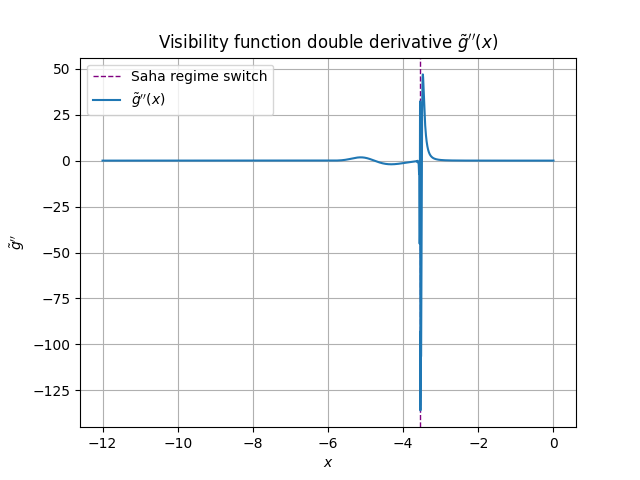
\includegraphics[width=0.4\textwidth]{../Milestone 2/Plots/g_tilde_double_deriv.png}
\caption{Second derivative of the visibility function. This one looks weird, especially the early bump around $x=-5$.}
\label{fig:milestone_2_g_tilde_double_deriv}
\end{figure}
